\documentclass[aspectratio=169,usenames,dvipsnames]{beamer}
\beamertemplatenavigationsymbolsempty
% \documentclass{beamer}

% UNCOMMENT FOR HANDOUTS
% \usepackage{pgfpages}
% \pgfpagesuselayout{2 on 1}[landscape,letterpaper,border shrink=5mm]
% \setbeameroption{show notes}

\mode<presentation>
\usetheme{Boadilla}
\usecolortheme{spruce}
\usepackage{../../LizStyle,ulem}
\usepackage{color}
\usepackage[color,matrix,arrow]{xy}
% \input xy
% \xyoption{all}
\usepackage{tikz}
\usepackage{tikz-cd}
\tikzset{commutative diagrams/diagrams={ampersand replacement=\&}}

\AtBeginSection{\frame{\sectionpage}}


% ==========Command for putting comments and removing them=======
% Visible:
\newcommand{\InstructorNotes}[1]{\textit{\color{orange}#1}}
\newcommand{\InstructorList}[1]{
\begin{itemize}
	\color{orange}
	#1
\end{itemize}
}
% Removed:
% \renewcommand{\InstructorNotes}[1]{}
% \renewcommand{\InstructorList}[1]{}


\newcommand{\bvfill}{\vskip0pt plus 1filll}

\usepackage{multimedia}
\usepackage{graphbox}

% \usepackage{algpseudocode}


\newcommand{\Reeb}{\textbf{Reeb}}
\newcommand{\Rtopc}{\textbf{Rtopc}}
% \newcommand{\RR}{\mathcal{R}}

\newcommand{\Set}{\textbf{Set}}
\newcommand{\Vect}{\textbf{Vect}}
\newcommand{\Top}{\textbf{Top}}
\newcommand{\Int}{\textbf{Int}}


\graphicspath{ {Figures/} {../../Figures/} }



\begin{document}
%\pdfoptionpdfminorversion 5
%\logo{\includegraphics[height=1.5cm]{dukeshield.pdf}}
\title[Review day]{Test 1 review day}
\subtitle{CMSE 381}
\date{Mon, Feb 10, 2025}



\institute[MSU-CMSE]{Michigan State University\\
			::\\
          Dept of Computational Mathematics, Science \& Engineering}
\author[Dr.~Zhang]{Prof.~Mengsen Zhang}

\begin{frame}
 \titlepage


\end{frame}
%--------------------------
\begin{frame}[c]{Announcements}

\begin{columns}

\column{.60\textwidth}
\centering

	Announcements: 
	\begin{itemize}
		\item midterm \# 1 on Wednesday
		\item Project info, honors option posted on \href{https://msu-cmse-courses.github.io/CMSE381-S25/Project/ProjectDescription.html}{course website}
	\end{itemize}
\end{columns}

\end{frame}
%--- Next Frame ---%
\begin{frame}[c]{Based on the questions submitted}

\begin{columns}
\column{.4\textwidth}
\centering
\begin{itemize}
	\item Bias Variance Trade off
	\item KNN classification
	\item How to prepare
	% \item Error rate (classification)
	% \item Bayes Classifier
	% \item $K$-NN classification
\end{itemize}
\column{.4\textwidth}
\centering

\end{columns}

\end{frame}
%--- Next Frame ---%

\begin{frame}[t]{Training error vs test error}
	\centering
	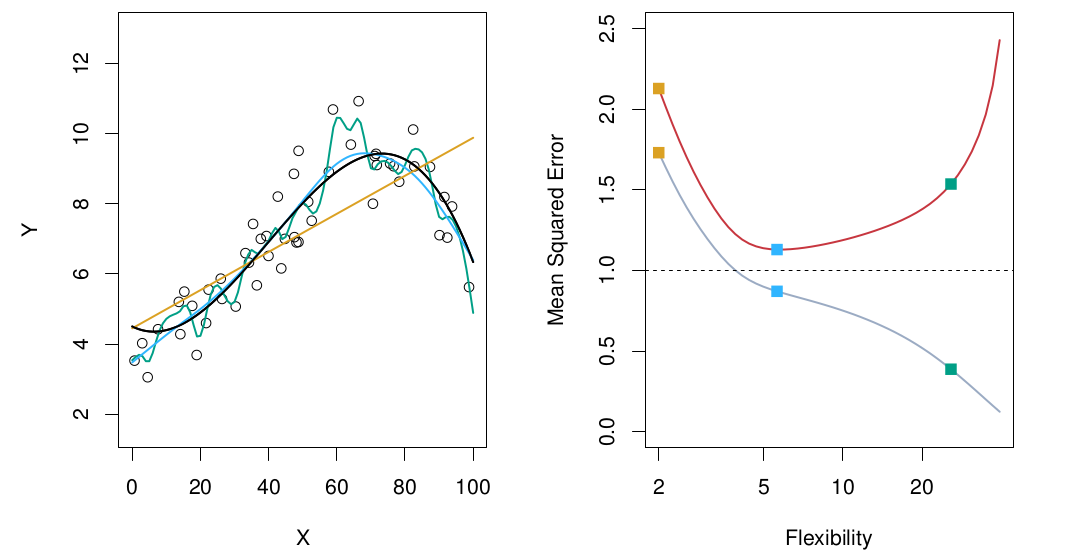
\includegraphics[width = .7\textwidth]{Fig2-9.png}


\tiny
	\InstructorList{
	\item Left: Black line is model for simulation of data
	\item Right side: training in blue/grey, testing in red
	\item Variance of $\e$ is dashed line
	\item Point out that training error goes down but test goes up (overfitting)
	\item Flexibility = degrees of freedom
	}
\end{frame}

\begin{frame}[t]{Bias-variance }

\begin{equation*}
	E(y_0 - \hat f (x_0))^2 = \Var(\hat f (x_0))
		+ \left[\mathrm{Bias}(\hat f(x_0)) \right] ^2
		+ \Var(\e)
\end{equation*}
\begin{columns}
\column{.4\textwidth}
\centering
\InstructorList{
\item Proof outside of the scope of class
\item $E(y_0 - \hat f (x_0))^2$ is expected test MSE at $x_0$; avg test MSE if repeatedly estimated $f$ with lots of training sets and tested each at $x_0$
\item Computed by averaging $E(y_0 - \hat f (x_0))^2$  over all values in the test set
}
\column{.4\textwidth}
\centering
\InstructorList{
\item Eqn says we need an $\hat f$ with both low variance and low bias
\item Also says error is bounded below by irreduceable error $\Var(\e)$
}
\end{columns}


\end{frame}
%--- Next Frame ---%
\begin{frame}[c]{Variance}

\begin{columns}
\column{.45\textwidth}
% \centering
\textbf{Variance:} the amount by which $\hat f$ would change if we
estimated it using a different training data set.
\InstructorList{
\item High variance: small changes in training data result in large changes in $\hat f$.
\item Example right: green curve more flexible, but also small changes in data set could cause large changes in the computed model.
}
\column{.4\textwidth}
\centering
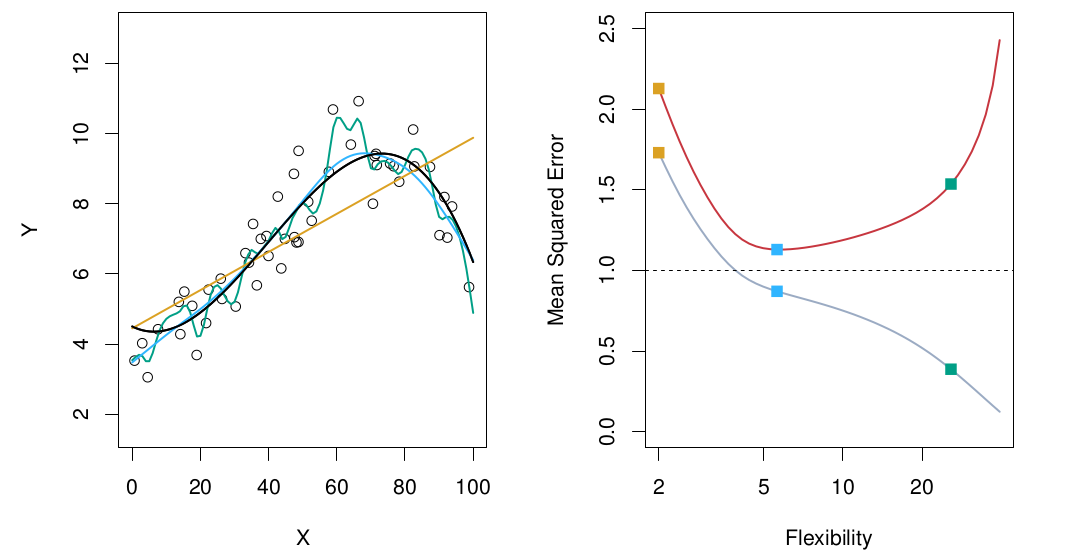
\includegraphics[width = \textwidth,clip, trim = 0 0 550 0 ]{Fig2-9}
\end{columns}

\end{frame}
%--- Next Frame ---%
\begin{frame}[t]{Bias}

\begin{columns}
\column{.45\textwidth}
% \centering

\textbf{Bias:} the error that is introduced by approximating a (complicated) real-life problem by a much simpler model.

% \tiny
\InstructorList{
\item Example: Linear regression, likely too simple for any real-life problem.
\item Figure at left: True $f$ is non-linear, so no good estimate possible with linear regression. (linear regression = high bias)
\item Figure at right: True $f$ is linear, so linear regression should do a good job (linear regression = low bias)
}
\column{.25\textwidth}
\centering
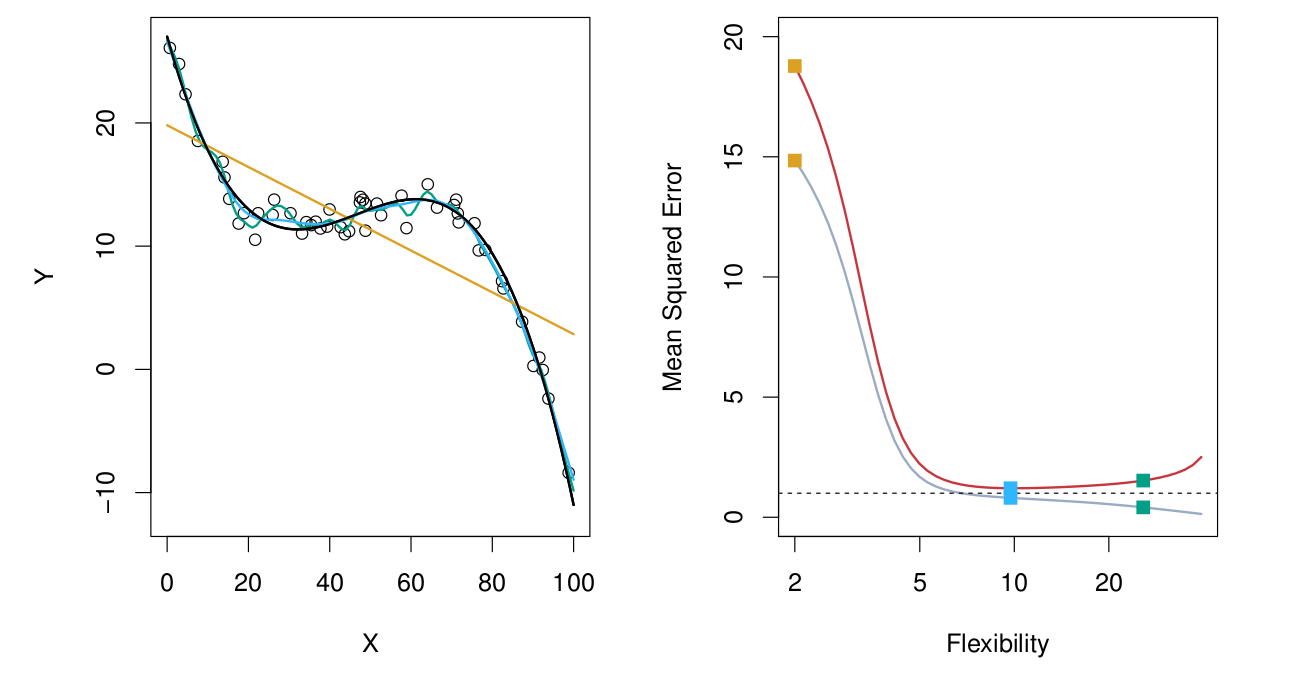
\includegraphics[width = \textwidth,clip, trim = 0 0 700 0 ]{Fig2-11}
\column{.25\textwidth}
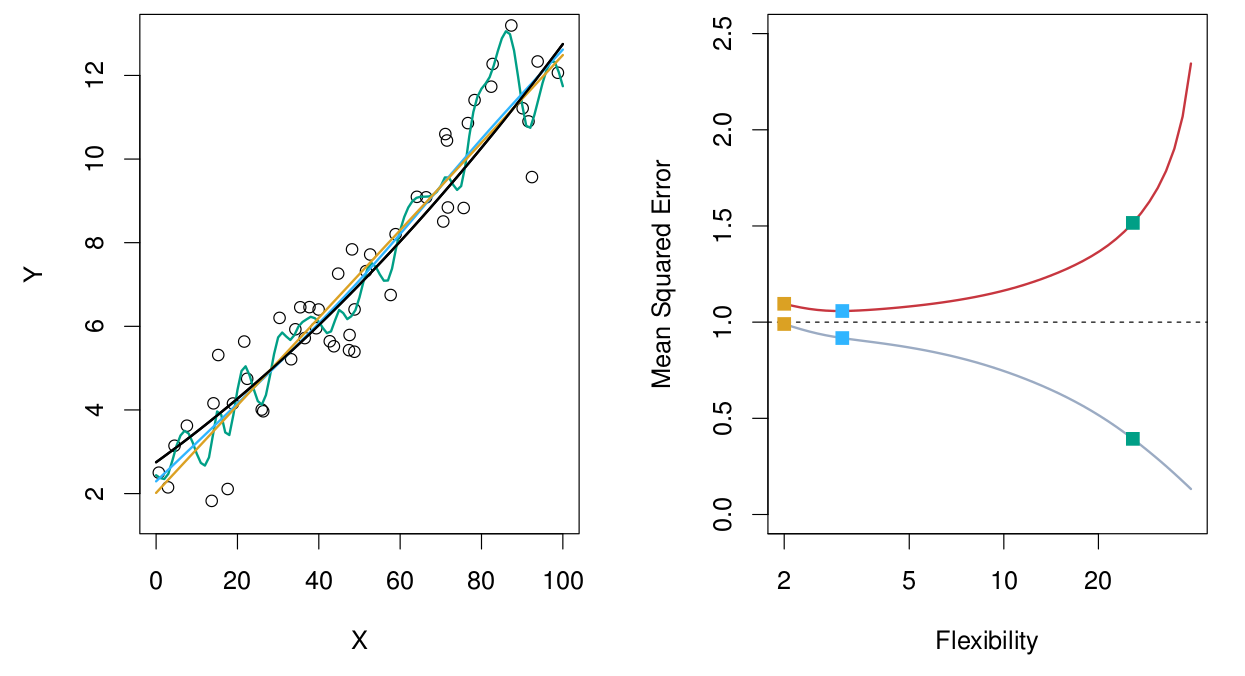
\includegraphics[width = \textwidth,clip, trim = 0 0 700 0 ]{Fig2-10}

\end{columns}

\end{frame}
%--- Next Frame ---%
{
  \setbeamercolor{background canvas}{bg=Apricot!25}
\begin{frame}[c]{Which is which}
	\bvfill
\begin{columns}
\column{.3\textwidth}
\centering
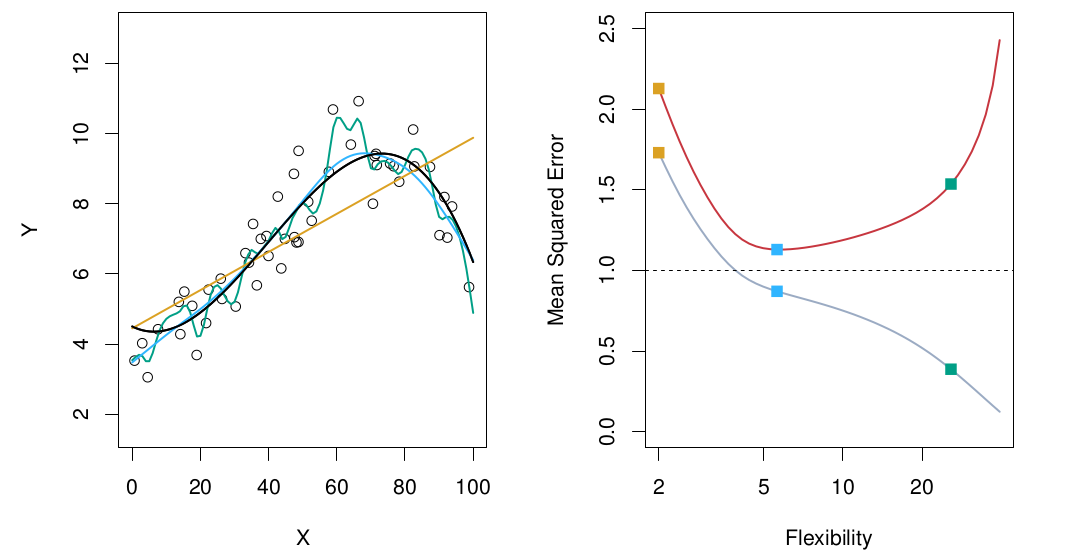
\includegraphics[width = \textwidth,clip, trim = 0 0 600 0 ]{Fig2-9}
\column{.3\textwidth}
\centering
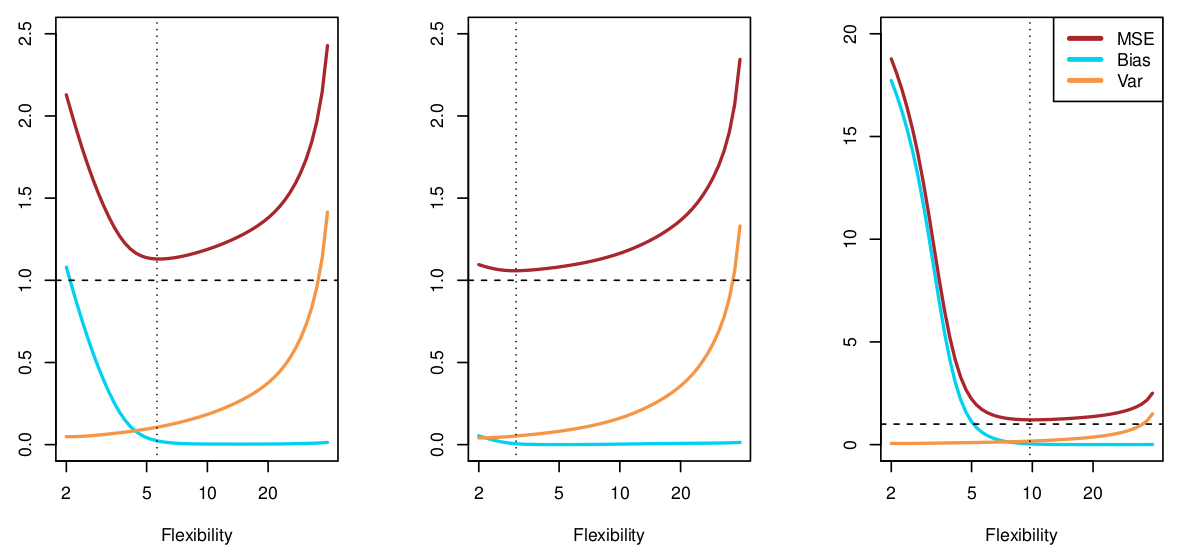
\includegraphics[width = .8\textwidth,clip, trim = 0 0 800 0 ]{Fig2-12}
\column{.3\textwidth}
Label the line corresponding to each of the following:
\begin{itemize}
	\item MSE 
	\item Bias 
	\item Variance of $\hat f(x_0)$
	\item Variance of $\e$
\end{itemize}
\end{columns}
	\bvfill
\begin{equation*}
	E(y_0 - \hat f (x_0))^2 = \Var(\hat f (x_0))
		+ \left[\mathrm{Bias}(\hat f(x_0)) \right] ^2
		+ \Var(\e)
\end{equation*}
\end{frame}
}

%--- Next Frame ---%
{
  \setbeamercolor{background canvas}{bg=Apricot!25}
\begin{frame}[t]{Review KNN classifier example}
Here label is shown by O vs X. What are the knn predictions for points $A$, $B$ and $C$ for $k=1$ or $k=3$? \InstructorNotes{Next year, maybe make an example like this with more than two levels, and/or try to decide what locations get which predictions for k=1 in prep for the next slide}
\begin{columns}
\column{.4\textwidth}
\centering

\includegraphics[align = c, width = \textwidth]{KNN-Example}

\column{.45\textwidth}
\centering
\begin{tabular}{c||c|c}
	               & $k=1$ & $k=3$ \\
	\textbf{Point} & Prediction & Prediction\\
	\hline 
	&& \\
	A &\InstructorNotes{O}& \InstructorNotes{O}\\
	&& \\
	B &\InstructorNotes{X}& \InstructorNotes{X}\\
	&& \\
	C &\InstructorNotes{O}& \InstructorNotes{X}\\
	&& \\
\end{tabular}
\InstructorNotes{
\includegraphics[align = c, width = .2\textwidth]{KNN-Example-Soln-K1}
\includegraphics[align = c, width = .2\textwidth]{KNN-Example-Soln-K3}
}
\end{columns}
\end{frame}
}


\begin{frame}[t]{Preparing for exam}
	\begin{itemize}
		\item review slides
		\item write down key concepts equations on the cheatsheet, annotate them
		\item find pictures, equations, results tables you don't understand. bring to this class or read up in text book. 
	\end{itemize}
\end{frame}
\end{document}
